

\chapter{Gender-Specific Changes in Treatment-Seeking Around Admission}
\label{ch:paper2}


%----------------------------------------------------------------%%----------------------------------------------------------------%


\vspace{0.5in}

\textbf{Paper:}
\textsc{\underline{Andreas H\"ohn}, Jutta Gampe, Rune Lindahl-Jacobsen, 
	    Kaare Christensen, and Anna Oksuzyan:} 
		Do men avoid seeking medical advice? A register-based study of 
		gender-specific changes in primary healthcare use after first 
		hospitalization at ages 60+ in Denmark. \textbf{\textit{submitted 
		to a peer-reviewed journal}}


%----------------------------------------------------------------%%----------------------------------------------------------------%


%%% ABSTRACT %%%

\newpage

\section{Abstract}
% BACKGROUND %
\textbf{Background:} It remains unclear whether women's greater primary healthcare 
use reflects a lower threshold for treatment-seeking or a health disadvantage. We 
address this question by studying primary healthcare use surrounding a major health 
shock.\\
% METHODS %
\textbf{Methods:} This cohort study utilized routinely-collected healthcare data 
covering the total Danish population aged 60+ between 1996 and 2011. Using a hurdle 
model, we investigated levels of primary healthcare use and levels of non-use before 
and after the first inpatient hospital admission for stroke, myocardial infarction (MI), 
chronic obstructive pulmonary disease (COPD), and gastrointestinal cancers (GIC).\\
% RESULTS %
\textbf{Results:} Before hospitalization, men were more likely to be non-users (Odds 
Ratios (ORs) \& 95\% Confidence Interval (CI); Stroke: 1.802 (1.731-1.872); MI: 1.841 
(1.760-1.922); COPD: 2.160 (2.028-2.292); GIC: 1.609 (1.525-1.693)), and had fewer 
contacts when they were users (Proportional Change ($\mathrm{e}^\beta$) \& 95\% CI; Stroke: 0.821 
(0.806-0.836); MI: 0.796 (0.778-0.814); COPD: 0.855 (0.832-0.878); GIC: 0.859 
(0.838-0.881)). Levels of non-use dropped more sharply among men (ORs \& 95\% CI; 
Stroke: 0.965 (0.879-1.052); MI: 0.894 (0.789-0.999); COPD: 0.755 (0.609-0.900); 
GIC: 0.895 (0.801-0.988)), and increases in the level of healthcare use were more  
pronounced among men users ($\mathrm{e}^\beta$ \& 95\% CI; Stroke: 1.113 (1.102-1.124); MI: 1.112 
(1.099-1.124); COPD: 1.078 (1.063-1.093); GIC: 1.097 (1.079-1.114)). Gender differences 
became more apparent after controlling for survival following hospitalization.\\
% CONCLUSION %
\textbf{Conclusion:} Women's consistently higher levels of primary healthcare use are 
likely to be explained by a combination of both: a lower threshold for seeking medical 
advice, and a health disadvantage resulting from better survival in bad health.\\


%----------------------------------------------------------------%%----------------------------------------------------------------%


\newpage

\section{Key Messages}

\begin{itemize}
	\item	The use of primary healthcare services increased sharply after an 
			admission to hospital among both men and women, pointing towards 
			a need-driven change in treatment-seeking in response to a health 
			shock.
	\item	Changes in the propensity to seek medical treatment after hospitalization 
			were more pronounced among men when compared to women suggesting that men 
			were more reluctant to engage with primary healthcare before hospitalization. 
			However, gender differences in primary healthcare use did not disappear 
			after admission to hospital.
	\item	Our findings indicate a lower threshold for treatment-seeking among women, 
			which is likely to be underpinned by women's better survival with disabling 
			conditions.
	\item	Attention should be given to increasing the use of primary healthcare 
			services in order to prevent and postpone acute episodes of health deterioration, 
			particularly among men.
\end{itemize}


%----------------------------------------------------------------%%----------------------------------------------------------------%


\newpage

\section{Background}

Women have lower mortality rates than men following most adverse health 
conditions, including hospitalizations.\citep{wang2016global,zarulli2018women,
hohn2018sex} To explain women's mortality advantage, the literature points 
towards the interaction of biological and behavioral factors.\citep{oksuzyan2008,
rieker2005rethinking} One observation among the behavioral factors is that 
women, on average, utilize primary healthcare more than men.\citep{banks2013men,
juel2008men} Primary healthcare is among the main means of prevention, and 
timely diagnosis can be crucial for effective treatment and prolonging an 
individual's life.\citep{olesen2009delay,starfield2005contribution}

Seeking medical help is a complex process, shaped by demographic, structural 
and individual factors such as age, gender, access to healthcare, socioeconomic 
inequalities, cultural norms, gender roles, and education.\citep{llanwarne2017wasting,
koefoed2013influence,gallagher2010symptoms,maclean2010rules} Most quantitative 
research documenting patterns in primary healthcare use is based on cross-sectional 
analysis of aggregate-level data. These findings have consistently shown that 
women utilize primary healthcare services more often than same-aged men -- even 
when excluding consultations for child-bearing and birth control.\citep{juel2008men,
wang2013men}  In contrast to population-level studies, individual-level studies 
have yielded mixed findings. Some studies report small or non-significant 
differences when comparing men and women who face similar conditions, such 
as headache, back pain, and prior major cancers.\citep{hunt2011women,wang2014gender,
vos2012does} Other studies have found consistently higher female use of primary 
healthcare when controlling for morbidity levels.\citep{jatrana2009gender,
lyratzopoulos2012variation,fridgen2013help,chang2009gender} It therefore 
remains unclear whether higher rates of primary healthcare use among women 
are due to a lower threshold for seeking medical help or whether they are 
due to women's health disadvantage.\citep{hunt2011women,case2005sex} In 
addition, studies have not distinguished between users and non-users of 
primary healthcare. This distinction is important because there may be no, 
or only small, differences in treatment-seeking behavior between women and 
those men who are willing to engage with healthcare. It may also be the case 
that gender differences in mean levels of primary healthcare use are primarily 
driven by gender differences in the share of non-users.

We investigated trajectories of primary healthcare use and levels of non-use 
surrounding a major health shock, defined as the first hospital admission at 
age 60 and older. We examined primary healthcare use patterns before and after 
hospitalization for four major causes of admission: stroke, myocardial infarction 
(MI), chronic obstructive pulmonary disease (COPD), and gastrointestinal cancers 
(GIC). We expected the frequency of contacts with primary healthcare to be higher 
in the period after admission to hospital, and to be generally higher among women. 
If men are more reluctant to seek medical advice until the occurrence of health 
shock, we may expect to see a greater change in primary healthcare use among men 
than among women following hospitalization.\\


%----------------------------------------------------------------%
%----------------------------------------------------------------%



\section{Methods}

\subsection{Data}
We utilized routinely-collected, population-based register data on hospital 
admissions and contacts with primary healthcare covering the entire Danish 
population. Using the unique personal identification number (CPR-Number), 
we linked records from the Central Population Registry (CPR), the National 
Patient Register (NPR), and the National Health Service Register (NHSR). 
While the CPR contains information on each resident's vital status, gender, 
and date of birth,\citep{pedersen2011,schmidt2014} the NPR contains 
information on hospital treatments since 1977, including dates of admission 
and discharge, and the causes of admission.\citep{lynge2011} The NHSR, 
established in 1990, contains data on primary healthcare use and includes 
information on the provider and a code for the provided services.\citep{sahl2011danish} 
Since treatments of under 16-year-olds were reported with the CPR-Number 
of one parent until 31 December 1995, we restricted our study period to 
1996--2014.\\

\subsection{Study Population}
Over one million men and women were aged 60 or older in Denmark by 1 January, 
1999 (N=1,056,733). We focused on healthcare use after age 60 to remove 
obstetrics-related healthcare use, which would otherwise have introduced 
a strong gender bias. We applied a 7-year washout-period to increase the 
likelihood that the observed admission is not a re-admission. Washout-periods 
of 7 years are recommended by the Swedish National Board of Health and Welfare 
in order to capture first events of MI,\citep{national2011myocardial} and 
have been widely used in register-based studies.\citep{karampampa2013trends,
modig2017estimating} We excluded 433,352 individuals who were admitted to 
hospital within the previous 7-year period, lasting from 1 January 1992 to 
31 December 1998.

Among the remaining individuals (N=623,381), we identified those who were 
admitted to a Danish hospital between 1 January, 1999 and 31 December, 2011 
(N=414,839). We defined an admission to hospital as the first inpatient hospital 
stay at age 60 or older, lasting three days (equivalent to two overnight stays) 
or longer, and distinguished whether the underlying cause for the hospitalization 
was stroke, MI, GIC, and COPD (N=65,622). We linked admissions with data on 
contacts with primary healthcare, covering the 33 months before and after 
hospitalization in order to capture changes in treatment-seeking behavior.

To account for a potential bias emerging from an increased healthcare use 
in close proximity to death,\citep{werblow2007population} we conducted a 
sensitivity check by restricting our analysis to those who survived the 
entire 33-month period following hospitalization. \\

\subsection{Study Design and Statistical Modeling}

The study design is illustrated in \hyperref[ch3:fig1]{Figure 1}. For each individual, we recorded 
the number of contacts with primary healthcare in five 6-month periods spanning 
30 months before and after the hospitalization event. To ensure that all intervals 
were of 6-month length, and to account for varying lengths of stay in hospital, 
we specified an additional interval surrounding the period of admission to hospital. 
This interval covered three months before and after hospitalization. We omitted 
this period from our analysis, and thus analyzed the frequency of contacts with 
primary healthcare in the five 6-month intervals preceding and following the 
6-month admission period. Consequently, the study period starts 33 months before 
admission and ends 33 months thereafter.\\

	%------------------%
	\begin{figure}[H]
		\centering
		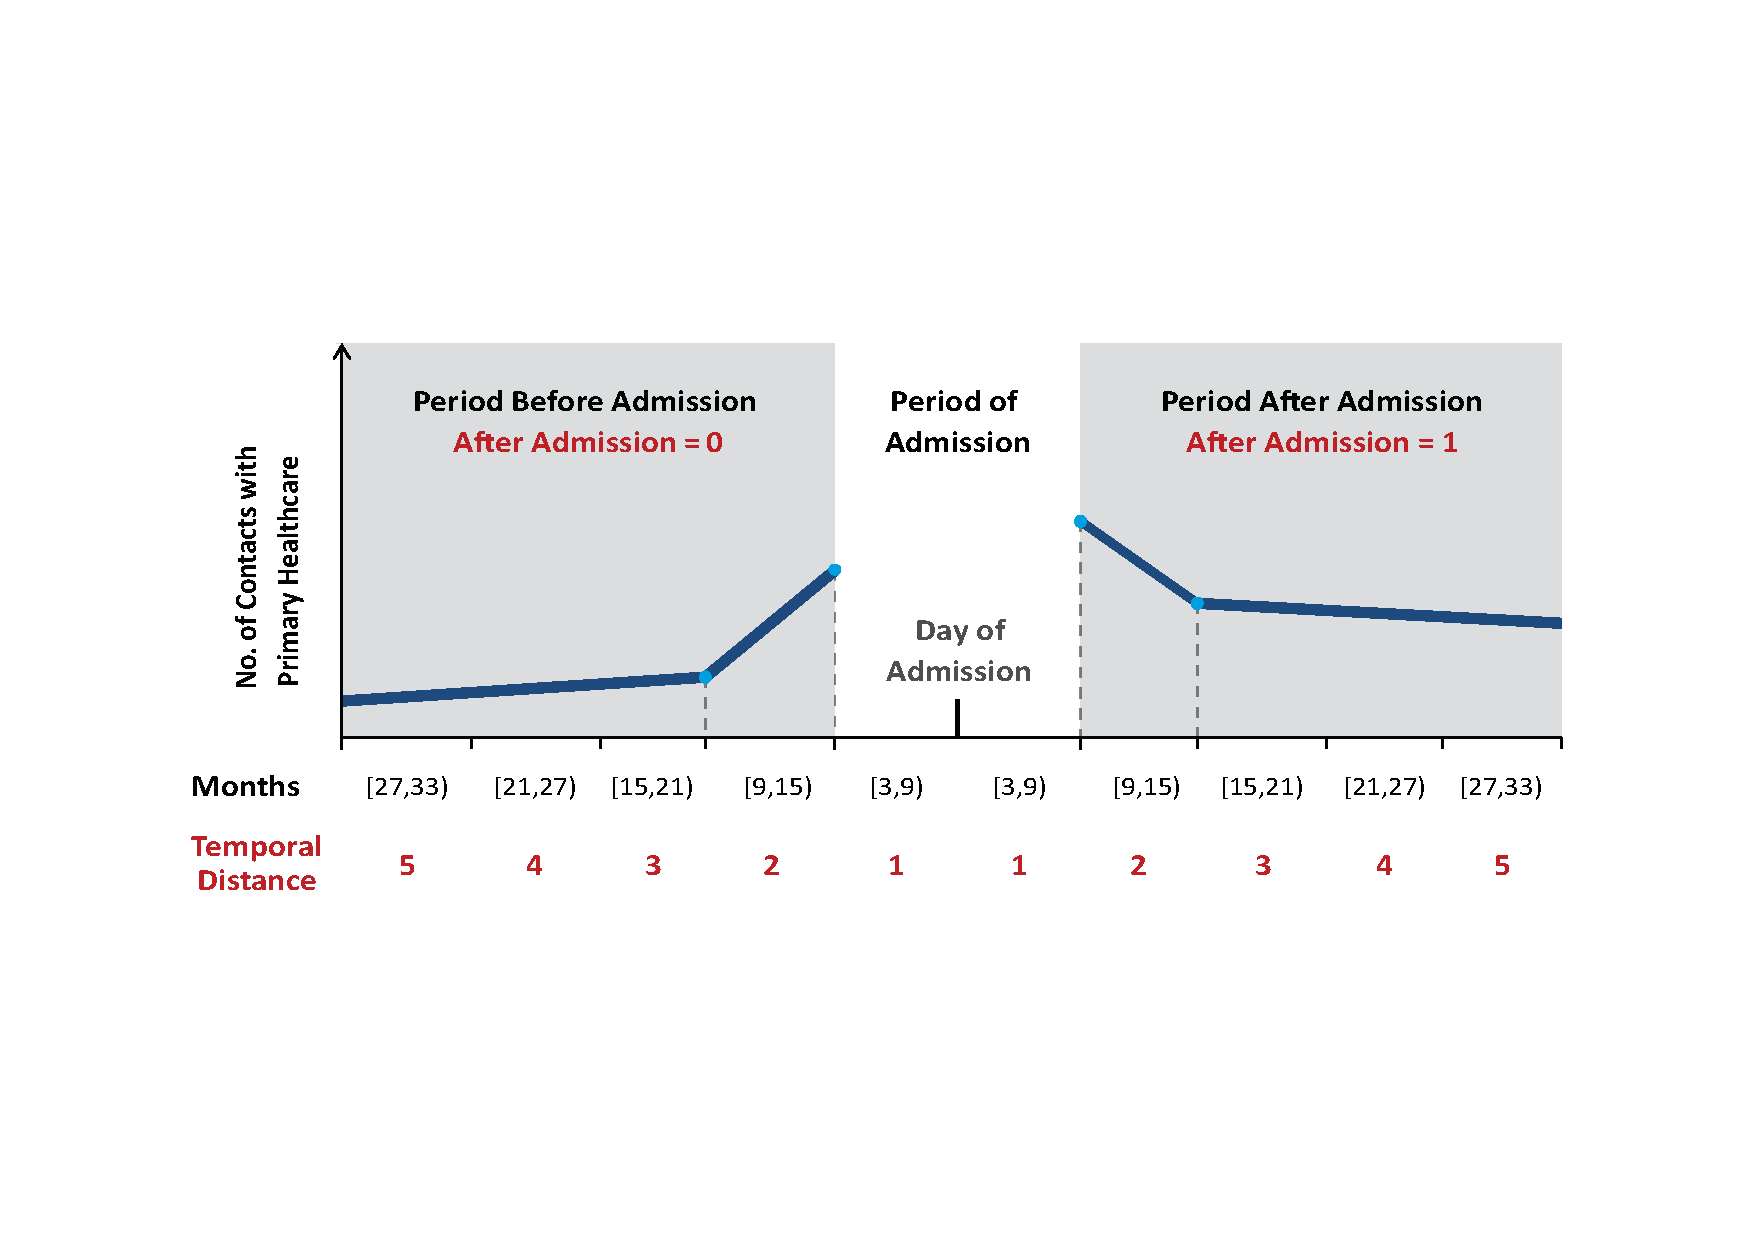
\includegraphics[scale=0.55]{Paper_2/MAIN_Figure_1.pdf}
		\caption*{\textbf{Figure 1:} 	Overview of the study design and the modeling 
										of time before and after hospital admission using 
										a linear spline.}
	\label{ch3:fig1}
	\end{figure}
	%--------------------%

We investigated how the number of contacts with primary healthcare changed 
with temporal distance to hospital admission (\textit{Temp.Dist.}) and other 
covariates. We introduced a binary variable (\textit{After}) that could, via 
interaction with \textit{Temp.Dist.}, capture potential differences in the 
trajectories of healthcare use before and after hospital admission.

In this longitudinal cohort study, the responses are repeated observations 
of counts. In addition, as shown in \hyperref[ch3:fig2]{Figure 2}, the marked zero-inflation 
present before hospital admission largely disappears thereafter. We therefore 
utilized a hurdle model to account for the special properties of our data.\citep{min2005random}

A hurdle model is a two-part model which combines a regression model for the 
probability of zero-counts with a regression model for the positive counts. The 
first part is a binomial logistic regression, which captures non-users of primary 
healthcare. The second part models the frequency of healthcare use for individuals 
who engage with primary healthcare. An individual random effect was incorporated 
to account for repeated observations. Positive counts were modeled by a truncated 
negative binomial regression with a log-link to account for overdispersion not 
captured by the observed covariates.\\

	%------------------%
	\begin{figure}[H]
		\centering
		\includegraphics[scale=0.6]{Paper_2/MAIN_Figure_2.pdf}
		\caption*{\textbf{Figure 2:} 	Distribution of contacts with primary 
										healthcare within the 3- to 9-month period 
										before and after admission to hospital.}
	\label{ch3:fig2}
	\end{figure}
	%--------------------%

As shown in \hyperref[ch3:tab1]{Table 1}, we performed model selection for both parts of the model 
step-wise and hierarchically, separately for each cause.\footnote{\textit{Note: 
$(1|ID)$ stands for individual random effect}} Temporal distance to hospitalization 
was included in two ways: either with a single linear effect (log-scale) or as 
a linear spline (lin.spl.), a piecewise-linear function, with a knot at \textit{Temp.Dist. = 2}. 
The linear spline allowed the slope to be different for the 6-month intervals next 
to the admission period as the healthcare use might change more rapidly close 
to admission. Using Akaike's Information Criterion (AIC), we selected Model 5 
as the final model. Parameter estimates are presented as Odds Ratios (OR) for 
the logistic model and as Proportional Change ($\mathrm{e}^\beta$) for the 
count model. Delta method was used to estimate 95\% confidence intervals (CI). 
The merging of registers was carried out with Stata (Version 14). Statistical 
models were estimated using the glmmTMB package for R (Version 3.5.1).\citep{brooks2017modeling} 


\begin{landscape}


\begin{table}[htbp]
  \centering
  \small
  \caption*{\textbf{Table 1:}	 Overview on the stepwise model development process; 
  								 models were developed separately by cause of admission}
    \begin{tabular}{ccclrrr}
    \toprule
    \textbf{Cause} & \textbf{M} & \textbf{Model for zero-counts} & \multicolumn{1}{c}{\textbf{Model for positive counts}} & \multicolumn{1}{c}{\textbf{AIC}} & \multicolumn{1}{c}{\textbf{dAIC}} & \multicolumn{1}{c}{\textbf{DF}} \\
    \midrule
    Stroke & 1     & After + Gender + Age + $(1|ID)$ & Temp.Dist. * After + Gender + Age + $(1|ID)$ & 1,014,319 & 753   & 17 \\
    Stroke & 2     & After + Gender + Age + $(1|ID)$ & Temp.Dist. * After + Gender * After + Age + $(1|ID)$ & 1,013,961 & 395   & 18 \\
    Stroke & 3     & After + Gender + Age + $(1|ID)$ & lin.spl.(Temp.Dist.) * After + Gender + Age + $(1|ID)$ & 1,013,925 & 359   & 19 \\
    Stroke & 4     & After + Gender + Age + $(1|ID)$ & lin.spl.(Temp.Dist.) * After + Gender * After + Age + $(1|ID)$ & 1,013,566 & 0     & 20 \\
    Stroke & 5     & After * Gender + Age + $(1|ID)$ & lin.spl.(Temp.Dist.) * After + Gender * After + Age + $(1|ID)$ & 1,013,567 & 1     & 21 \\
    MI    & 1     & After + Gender + Age + $(1|ID)$ & Temp.Dist. * After + Gender + Age + $(1|ID)$ & 719,204 & 468   & 17 \\
    MI    & 2     & After + Gender + Age + $(1|ID)$ & Temp.Dist. * After + Gender * After + Age + $(1|ID)$ & 718,932 & 195   & 18 \\
    MI    & 3     & After + Gender + Age + $(1|ID)$ & lin.spl.(Temp.Dist.) * After + Gender + Age + $(1|ID)$ & 719,012 & 275   & 19 \\
    MI    & 4     & After + Gender + Age + $(1|ID)$ & lin.spl.(Temp.Dist.) * After + Gender * After + Age + $(1|ID)$ & 718,739 & 2     & 20 \\
    MI    & 5     & After * Gender + Age + $(1|ID)$ & lin.spl.(Temp.Dist.) * After + Gender * After + Age + $(1|ID)$ & 718,737 & 0     & 21 \\
    COPD  & 1     & After + Gender + Age + $(1|ID)$ & Temp.Dist. * After + Gender + Age + $(1|ID)$ & 447,466 & 176   & 17 \\
    COPD  & 2     & After + Gender + Age + $(1|ID)$ & Temp.Dist. * After + Gender * After + Age + $(1|ID)$ & 447,368 & 79    & 18 \\
    COPD  & 3     & After + Gender + Age + $(1|ID)$ & lin.spl.(Temp.Dist.) * After + Gender + Age + $(1|ID)$ & 447,399 & 110   & 19 \\
    COPD  & 4     & After + Gender + Age + $(1|ID)$ & lin.spl.(Temp.Dist.) * After + Gender * After + Age + $(1|ID)$ & 447,302 & 12    & 20 \\
    COPD  & 5     & After * v + Age + $(1|ID)$ & lin.spl.(Temp.Dist.) * After + Gender * After + Age + $(1|ID)$ & 447,289 & 0     & 21 \\
    GIC   & 1     & After + Gender + Age + $(1|ID)$ & Temp.Dist. * After + Gender + Age + $(1|ID)$ & 513,393 & 274   & 17 \\
    GIC   & 2     & After + Gender + Age + $(1|ID)$ & Temp.Dist. * After + Gender * After + Age + $(1|ID)$ & 513,289 & 169   & 18 \\
    GIC   & 3     & After + Gender + Age + $(1|ID)$ & lin.spl.(Temp.Dist.) * After + Gender + Age + $(1|ID)$ & 513,228 & 109   & 19 \\
    GIC   & 4     & After + Gender + Age + $(1|ID)$ & lin.spl.(Temp.Dist.) * After + Gender * After + Age + $(1|ID)$ & 513,123 & 3     & 20 \\
    GIC   & 5     & After * Gender + Age + $(1|ID)$ & lin.spl.(Temp.Dist.) * After + Gender * After + Age + $(1|ID)$ & 513,119 & 0     & 21 \\
    \bottomrule
    \bottomrule
    \end{tabular}%
\label{ch3:tab1}
\end{table}%


\end{landscape}


%----------------------------------------------------------------%


\section{Results}

\subsection{Descriptive Statistics}
As shown in \hyperref[ch3:tab2]{Table 2}, we studied 65,622 individuals, of whom 48\% were women 
and 52\% were men. The mean age at first admission was significantly higher 
(p-Value $<$ 0.001) among women (77.25 years) than men (75.17 years). \\

%----------------------------------------------------------------%

%%% TABLE 2 %%%
\begin{table}[htbp]
  \centering
  \caption*{\textbf{Table 2:} 	Number and percentage of hospital admissions by 
  								gender and cause of admission to hospital.}
 \begin{tabular}{cp{7.57em}cccc}
    \toprule
    \textbf{Cause of } & \textbf{ICD-10} & \multicolumn{2}{c}{\textbf{Men }} & \multicolumn{2}{c}{\textbf{Women }} \\
    \textbf{Admission} & \textbf{Chapter} & \textbf{No.} & \textbf{in \%} & \textbf{No. } & \textbf{in \%} \\
    \midrule
    Stroke  & I.61 -- I.64 & 11,919 & 34.8  & 12,227 & 38.9 \\
    MI    & I.21 -- I.22 & 10,482 & 30.6  & 6,736 & 21.4 \\
    COPD  & J.40 -- J.47 & 4,335 & 12.7  & 5,530 & 17.6 \\
    GIC   & C.15 -- C.26 & 7,465 & 21.8  & 6,928 & 22 \\
    \midrule
    \textbf{Total} & \textbf{-} & \textbf{34,201} & \textbf{100} & \textbf{31,421} & \textbf{100} \\
    \bottomrule
    \end{tabular}%
\label{ch3:tab2}
\end{table}%

%----------------------------------------------------------------%


\subsection{Regression Model}
The estimated hurdle models are shown in \hyperref[ch3:tab3]{Table 3}. The upper 
section of \hyperref[ch3:tab3]{Table 3} shows the model for being in the non-user 
group. Before hospitalization, we found that men had higher odds of being in the 
non-user group than women (ORs \& 95\% CI; Stroke: 1.802 (1.731-1.872); MI: 1.841 
(1.760-1.922); COPD: 2.160 (2.028-2.292); GIC: 1.609 (1.525-1.693); all p-Values 
$<$ 0.001). For men and women, and across all causes, the odds of being in the 
non-user group were consistently smaller in the period after admission than in 
the period before admission (ORs \& 95\% CI; Stroke: 0.062 (0.000-0.129); MI: 
0.074 (0.000-0.163); COPD: 0.190 (0.087-0.293); GIC: 0.230 (0.159-0.301); all 
p-Values $<$ 0.001). The interaction effect between gender and the period after 
hospitalization suggests that, after hospital admission, the decline in the probability 
of being a non-user was larger among men than women for all causes apart from 
stroke (ORs \& 95\% CI; Stroke: 0.965 (0.879-1.052), p-Value: 0.420; MI: 0.894 
(0.789-0.999), p-Value: 0.036; COPD: 0.755 (0.609-0.900), p-Value: 0.001; GIC: 
0.895 (0.801-0.988), p-Value: 0.020).

Translated into probabilities, this means that levels of non-use were substantially 
smaller in the period after hospitalization, and that gender differences in 
the probability of being a non-user were smaller in the period after, than 
in the period before hospitalization. For example, a man aged 60-69, who 
was admitted for MI, had a 25\% probability of being in the non-user group 
before admission, while the probability among women was 15\%. After admission 
for MI, the corresponding probabilities of non-use were 2\% among men and 1\% 
among women.

The lower section of \hyperref[ch3:tab3]{Table 3} shows the regression results for the positive 
counts model. Across all causes of admission, we found that the average 
number of contacts with primary healthcare increased steadily before 
hospitalization. Within the period before admission, men had less contact 
when compared to women ($\mathrm{e}^\beta$ \& 95\% CI; Stroke: 0.821 
(0.806-0.836); MI: 0.796 (0.778-0.814); COPD: 0.855 (0.832-0.878); GIC: 
0.859 (0.838-0.881); all p-Values $<$ 0.001).

The average number of contacts with primary healthcare jumped in level 
after hospitalization. This increase was higher for the conditions, stroke 
and MI, when compared with the conditions COPD and GIC ($\mathrm{e}^\beta$ 
\& 95\% CI; Stroke: 1.727 (1.715-1.739); MI: 1.638 (1.624-1.652); COPD: 
1.291 (1.275-1.307); GIC: 1.350 (1.331-1.368); all p-Values $<$ 0.001). 
However, the post-hospitalization increase in the average number of contacts 
was larger among men than among women ($\mathrm{e}^\beta$ \& 95\% CI; Stroke: 
1.113 (1.102-1.124); MI: 1.112 (1.099-1.124); COPD: 1.078 (1.063-1.093); 
GIC: 1.097 (1.079-1.114); all p-Values $<$ 0.001). Gender differences 
among users of primary healthcare were therefore smaller in the period 
after than in the period before hospital admission. Nevertheless, level 
differences between men and women of the user group did not fully disappear 
after hospitalization.

%----------------------------------------------------------------%


\begin{landscape}

\begin{table}[H]
  \scriptsize
  \centering
  \caption*{\textbf{Table 3:} Results of hurdle regression models.}
    \begin{tabular}{lcccccccc}
    \toprule
    \textbf{Log. Model } & \multicolumn{2}{c}{\textbf{Stroke}} & \multicolumn{2}{c}{\textbf{MI}} & \multicolumn{2}{c}{\textbf{COPD}} & \multicolumn{2}{c}{\textbf{GIC}} \\
    \textbf{for Zero Counts } & \textbf{Est. (95\%CI)} & \textbf{p-Value} & \textbf{Est. (95\%CI)} & \textbf{p-Value} & \textbf{Est. (95\%CI)} & \textbf{p-Value} & \textbf{Est. (95\%CI)} & \textbf{p-Value} \\
    \midrule
    Intercept & 0.173 (0.083-0.262) & $<$0.001 & 0.178 (0.084-0.273) & $<$0.001 & 0.027 (0.000-0.193) & $<$0.001 & 0.217 (0.121-0.314) & $<$0.001 \\
          &       &       &       &       &       &       &       &  \\
    After  & 0.062 (0.000-0.129) & $<$0.001 & 0.074 (0.000-0.163) & $<$0.001 & 0.190 (0.087-0.293) & $<$0.001 & 0.230 (0.159-0.301) & $<$0.001 \\
          &       &       &       &       &       &       &       &  \\
    Men   & 1.802 (1.731-1.872) & $<$0.001 & 1.841 (1.760-1.922) & $<$0.001 & 2.160 (2.028-2.292) & $<$0.001 & 1.609 (1.525-1.693) & $<$0.001 \\
    Men*After  & 0.965 (0.879-1.052) & 0.42  & 0.894 (0.789-0.999) & 0.036 & 0.755 (0.609-0.900) & 0.001 & 0.895 (0.801-0.988) & 0.02 \\
          &       &       &       &       &       &       &       &  \\
    Age 70-79 & 0.528 (0.438-0.619) & $<$0.001 & 0.465 (0.375-0.555) & $<$0.001 & 0.597 (0.444-0.751) & $<$0.001 & 0.458 (0.360-0.557) & $<$0.001 \\
    Age 80-89 & 0.347 (0.247-0.446) & $<$0.001 & 0.278 (0.170-0.386) & $<$0.001 & 0.435 (0.244-0.626) & $<$0.001 & 0.287 (0.168-0.407) & $<$0.001 \\
    Age 90+ & 0.321 (0.143-0.499) & $<$0.001 & 0.265 (0.049-0.480) & $<$0.001 & 0.658 (0.134-1.183) & 0.118 & 0.230 (0.000-0.538) & $<$0.001 \\
    \midrule
          &       &       &       &       &       &       &       &  \\
    \midrule
    \textbf{NB Model} & \multicolumn{2}{c}{\textbf{Stroke}} & \multicolumn{2}{c}{\textbf{MI}} & \multicolumn{2}{c}{\textbf{COPD}} & \multicolumn{2}{c}{\textbf{GIC}} \\
    \textbf{for Positive Counts} & \textbf{Est. (95\%CI)} & \textbf{p-Value} & \textbf{Est. (95\%CI)} & \textbf{p-Value} & \textbf{Est. (95\%CI)} & \textbf{p-Value} & \textbf{Est. (95\%CI)} & \textbf{p-Value} \\
    \midrule
    Intercept & 3.634 (3.615-3.654) & $<$0.001 & 3.535 (3.513-3.558) & $<$0.001 & 5.126 (5.101-5.152) & $<$0.001 & 3.463 (3.437-3.490) & $<$0.001 \\
          &       &       &       &       &       &       &       &  \\
    lin.spl.(Temp.Dist.)1 & 0.944 (0.933-0.955) & $<$0.001 & 0.948 (0.935-0.961) & $<$0.001 & 0.910 (0.896-0.925) & $<$0.001 & 0.871 (0.856-0.887) & $<$0.001 \\
    lin.spl.(Temp.Dist.)2 & 0.872 (0.861-0.884) & $<$0.001 & 0.877 (0.863-0.890) & $<$0.001 & 0.801 (0.787-0.816) & $<$0.001 & 0.787 (0.771-0.802) & $<$0.001 \\
    After & 1.727 (1.715-1.739) & $<$0.001 & 1.638 (1.624-1.652) & $<$0.001 & 1.291 (1.275-1.307) & $<$0.001 & 1.350 (1.331-1.368) & $<$0.001 \\
    lin.spl.(Temp.Dist.)1*After  & 0.937 (0.922-0.951) & $<$0.001 & 0.944 (0.928-0.961) & $<$0.001 & 1.056 (1.037-1.075) & $<$0.001 & 1.062 (1.040-1.084) &$<$0.001 \\
    lin.spl.(Temp.Dist.)2*After  & 0.983 (0.968-0.998) & 0.023 & 0.955 (0.938-0.972) & $<$0.001 & 1.241 (1.221-1.261) & $<$0.001 & 1.166 (1.142-1.189) & $<$0.001 \\
          &       &       &       &       &       &       &       &  \\
    Men   & 0.821 (0.806-0.836) & $<$0.001 & 0.796 (0.778-0.814) & $<$0.001 & 0.855 (0.832-0.878) & $<$0.001 & 0.859 (0.838-0.881) & $<$0.001 \\
    Men*After & 1.113 (1.102-1.124) & $<$0.001 & 1.112 (1.099-1.124) & $<$0.001 & 1.078 (1.063-1.093) & $<$0.001 & 1.097 (1.079-1.114) & $<$0.001 \\
          &       &       &       &       &       &       &       &  \\
    Age 70-79 & 1.116 (1.097-1.135) & $<$0.001 & 1.143 (1.123-1.163) & $<$0.001 & 1.079 (1.053-1.105) & $<$0.001 & 1.132 (1.106-1.157) & $<$0.001 \\
    Age 80-89 & 1.161 (1.141-1.181) & $<$0.001 & 1.240 (1.217-1.263) & $<$0.001 & 1.097 (1.066-1.129) & $<$0.001 & 1.216 (1.187-1.246) & $<$0.001 \\
    Age 90+ & 1.129 (1.094-1.164) & $<$0.001 & 1.230 (1.186-1.274) & $<$0.001 & 1.070 (0.981-1.158) & 0.136 & 1.277 (1.206-1.348) & $<$0.001 \\
    \midrule
    \textit{No. of Observations} & \multicolumn{2}{c}{217,000} & \multicolumn{2}{c}{157,680} & \multicolumn{2}{c}{88,712} & \multicolumn{2}{c}{114,961} \\
    \textit{No. of Groups} & \multicolumn{2}{c}{24,146} & \multicolumn{2}{c}{17,218} & \multicolumn{2}{c}{9,865} & \multicolumn{2}{c}{14,393} \\
    \textit{VAR Ind. RE Log. Model} & \multicolumn{2}{c}{4.6} & \multicolumn{2}{c}{3.9} & \multicolumn{2}{c}{6.05} & \multicolumn{2}{c}{3.87} \\
    \textit{VAR Ind. RE NB Model} & \multicolumn{2}{c}{0.23} & \multicolumn{2}{c}{0.24} & \multicolumn{2}{c}{0.25} & \multicolumn{2}{c}{0.28} \\
    \textit{Overdisp. Par. NB Model} & \multicolumn{2}{c}{11.2} & \multicolumn{2}{c}{15.5} & \multicolumn{2}{c}{13.9} & \multicolumn{2}{c}{8.55} \\
    \bottomrule
    \end{tabular}%
\label{ch3:tab3}
\end{table}%

\end{landscape}


%----------------------------------------------------------------%


The trajectories of contacts with primary healthcare before and after 
hospitalization among men and women admitted for MI are shown in 
\hyperref[ch3:fig3]{Figure 3}. Visualizations for COPD, stroke, 
and GIC can be found in \hyperref[ch3:figS1]{Supplementary Figure S1},
\hyperref[ch3:figS2]{Supplementary Figure S2}, and
\hyperref[ch3:figS3]{Supplementary Figure S3 } at the end of this paper.\\

	%------------------%
	\begin{figure}[H]
		\centering
		\includegraphics[scale=0.425]{Paper_2/MAIN_Figure_3.pdf}
		\caption*{\textbf{Figure 3:} 	Estimated average number of contacts with 
										primary healthcare before and after admission 
										to hospital for MI.}
	\label{ch3:fig3}
	\end{figure}
	%--------------------%


\subsection{Sensitivity Analysis}
To examine the impact of mortality selection following hospitalization, 
we restricted the study population to all individuals who survived the 
33-month period after admission (N=42,683) and re-ran the analysis. We 
observed only marginal changes in the parameters of the hurdle models. 
However, before and after admission, gender differences in non-use and 
levels of primary healthcare use among users were consistently larger 
in this setting. This suggests that women's higher primary healthcare 
use around hospitalization is linked with their longer survival in 
poorer health when compared to men. Results of sensitivity analyses 
are shown in \hyperref[ch3:tabS1]{Supplementary Table S1}, 
\hyperref[ch3:tabS2]{Supplementary Table S2}, and
\hyperref[ch3:tabS3]{Supplementary Table S3 } at the end of this paper.\\

%----------------------------------------------------------------%%----------------------------------------------------------------%


\section{Discussion}

\subsection{Principal Findings}

We investigated patterns of primary healthcare use among men and women 
around the first hospital admission at ages 60+. Across all studied 
causes, men had lower levels of primary healthcare use before and 
after hospitalization. In addition, men had higher probabilities of 
being non-users -- especially before hospitalization. After experiencing 
a health shock, changes in primary healthcare use patterns, in particular 
the probability of being a non-user and the primary healthcare use 
levels, were more marked  among men than among women.\\

\subsection{Strengths and Limitations}

We utilized high-quality register data, which covered the entire Danish 
Population between 1992 and 2014. Working with population-based registers 
reduces the challenges of longitudinal surveys: losses to follow-up, recall 
bias, and non-responses. These often differ systematically between men and 
women, and may have a significant impact on the generalizability of 
findings.\citep{hunt2011women,oliver2005help}

We used individual-level data on four causes of hospital admission to 
examine changes in treatment-seeking behavior after a health shock, 
aiming for a comparison of men and women facing a similar health condition. 
Unfortunately, our data did not allow us to investigate the severity of 
the underlying conditions. Furthermore, the data on primary healthcare 
did not allow us to distinguish whether a contact was directly related 
to the cause of admission, and whether it was a preventative visit or 
for continuing treatment. In addition, our findings may be limited to 
healthcare contexts which are similar to the Danish with nationwide 
coverage for all residents and no out-of-pocket expenses for GP visits. 
Despite these limitations, our study makes an important contribution 
to the literature by examining gender differences in the levels of 
primary healthcare use in a longitudinal setting, across four major 
conditions, and by identifying users and non-users of primary 
healthcare.\\

\subsection{Interpretations and Implications}

Using a hurdle model enabled us to distinguish between two stochastic 
processes: first, the probability that individuals do not engage with 
primary healthcare, and second, the number of contacts for those individuals 
who are users of primary healthcare. This distinction is important 
as our analysis showed that, once men and women were users of primary 
healthcare, their general trajectories of healthcare use do not differ. 
It is therefore possible that gender differences in non-use might 
explain a substantial part of gender differences in mean levels of 
primary healthcare use on the population level.

Differentiating by cause of hospitalization allowed us to investigate 
whether gender differences in primary healthcare use varied across 
conditions. We found absolute gender differences in non-use and use 
levels to be largest across the acute conditions stroke and MI –-
conditions, for which symptoms might not be present before disease 
onset, or already-present symptoms might be overlooked. Contrastingly, 
for example, patients with COPD are likely to have noticeable symptoms 
long before admission. This is likely to explain why levels of non-use 
and the magnitude of absolute gender differences in both parts of the 
hurdle model were generally lowest among patients with COPD.

Before admission to hospital, and consistently across all four causes 
of admission, men were more likely to be non-users of primary healthcare 
than women. This finding  appears to be in line with early qualitative 
work on differentials in treatment-seeking behavior, which reported 
that the postponement of treatment-seeking is gender patterned.\citep{robertson2006not,
o2005s,smith2005patients,courtenay2000constructions} In the past, the 
over-generalization of these findings has contributed to over-simplified, 
stereotypical expectations about gender and treatment-seeking behavior: 
that men are more reluctant to seek medical advice, while women are 
over-users of the healthcare system, and are more willing to consult 
a doctor even with less-serious complaints.\citep{maclean2017does,
annandale2007gender} However, we found a remarkable share of 
women to be non-users of primary healthcare before admission to 
hospital. This is consistent with more recent work, which has 
demonstrated that neglecting symptoms and postponing treatment-seeking 
exist among women, too.\citep{maclean2017does} Therefore, 
treatment-seeking differentials should not be separated into 
binary gender patterns. Men and women may face similar psycho-social 
obstacles to using primary healthcare services.\citep{galdas2010help} 
For example, both genders may postpone seeing a doctor when no urgency 
is perceived.\citep{hunt2011women} At the same time, when experiencing 
signs of a severe disease, such as lung cancer, fear of the implications 
of a diagnosis may be a reason for not seeking medical advice.\citep{hamann2014stigma,
chambers2012systematic,scambler2009health} In our study, the probabilities 
of being a non-user of primary healthcare after admission to hospital were 
equally low among men and women. This may partly reflect the impact of 
established treatment schemes after hospitalization, which are fixed 
irrespective of gender. We interpret the higher post-hospitalization 
increase in primary healthcare use among men, in both parts of the 
hurdle model, to indicate that  men were more reluctant to seek medical 
advice before experiencing an acute health shock. Nevertheless, gender 
differences in contacts with primary healthcare did not fully disappear 
after hospitalization. This may be due to higher mortality selection in 
men following hospitalization: women are more likely to survive with 
disabling conditions.\citep{hohn2018sex}  Supporting this assumption, 
we found greater gender differences when restricting the analysis to 
individuals who survived the entire 33-month period following admission.\\

\subsection{Conclusion}
Our findings indicate a lower threshold for treatment-seeking among 
women. In addition, higher levels of primary healthcare use among women 
may be underpinned by the fact that women are more likely to survive 
with disabling conditions following hospitalization. Attention should 
be given to increasing men's and women's usage of primary healthcare 
services, long before hospitalization, to prevent or postpone the 
ultimate health deterioration.\\


%----------------------------------------------------------------%
%----------------------------------------------------------------%


\newpage


\section{Supplementary Material}


\subsection{Supplementary Figures}


	%------------------%
	\begin{figure}[H]
		\centering
		\includegraphics[scale=0.435]{Paper_2/SUPP_Figure_1_COPD.pdf}
		\caption*{\textbf{Supplementary Figure S1:} Estimated, average number of contacts with 
													primary healthcare before and after admission 
													to hospital for chronic obstructive pulmonary 
													disease (COPD).}
	\label{ch3:figS1}
	\end{figure}
	%--------------------%
	
	%------------------%
	\begin{figure}[H]
		\centering
		\includegraphics[scale=0.435]{Paper_2/SUPP_Figure_2_STROKE.pdf}
		\caption*{\textbf{Supplementary Figure S2:} Estimated, average number of contacts with 
													primary healthcare before and after admission 
													to hospital for stroke.}
	\label{ch3:figS2}
	\end{figure}
	%--------------------%
	
	%------------------%
	\begin{figure}[H]
		\centering
		\includegraphics[scale=0.435]{Paper_2/SUPP_Figure_3_GIC.pdf}
		\caption*{\textbf{Supplementary Figure S3:} Estimated, average number of contacts with 
													primary healthcare before and after admission 
													to hospital for gastrointestinal cancers (GIC).}
	\label{ch3:figS3}
	\end{figure}
	%--------------------%


%----------------------------------------------------------------%%----------------------------------------------------------------%


\newpage

	
\subsection{Supplementary Tables}


\begin{landscape}

%%% SUPP TABLE 1 %%%
\begin{table}[htbp]
  \centering
  \small
  \caption*{\textbf{Supplementary Table S1:}	Overview on the stepwise model development 
 												process; survivors of the 33-month study period.}    
  \begin{tabular}{ccclrrr}
    \toprule
    \textbf{Cause} & \textbf{M} & \textbf{Model for zero-counts } & \multicolumn{1}{c}{\textbf{Model for positive counts}} & \multicolumn{1}{c}{\textbf{AIC}} & \multicolumn{1}{c}{\textbf{dAIC}} & \multicolumn{1}{c}{\textbf{DF}} \\
    \midrule
    Stroke & 1     & After + Gender + Age + $(1|ID)$ & Temp.Dist. * After + Gender + Age + $(1|ID)$ & 783,611 & 753   & 17 \\
    Stroke & 2     & After + Gender + Age + $(1|ID)$ & Temp.Dist. * After + Gender * After + Age + $(1|ID)$ & 783,310 & 395   & 18 \\
    Stroke & 3     & After + Gender + Age + $(1|ID)$ & lin.spl.(Temp.Dist.) * After + Gender + Age + $(1|ID)$ & 783,224 & 359   & 19 \\
    Stroke & 4     & After + Gender + Age + $(1|ID)$ & lin.spl.(Temp.Dist.) * After + Gender * After + Age + $(1|ID)$ & 782,922 & 0     & 20 \\
    Stroke & 5     & After * Gender + Age + $(1|ID)$ & lin.spl.(Temp.Dist.) * After + Gender * After + Age + $(1|ID)$ & 782,923 & 1     & 21 \\
    MI    & 1     & After + Gender + Age + $(1|ID)$ & Temp.Dist. * After + Gender + Age + $(1|ID)$ & 585,568 & 452   & 17 \\
    MI    & 2     & After + Gender + Age + $(1|ID)$ & Temp.Dist. * After + Gender * After + Age + $(1|ID)$ & 585,347 & 231   & 18 \\
    MI    & 3     & After + Gender + Age + $(1|ID)$ & lin.spl.(Temp.Dist.) * After + Gender + Age + $(1|ID)$ & 585,342 & 225   & 19 \\
    MI    & 4     & After + Gender + Age + $(1|ID)$ & lin.spl.(Temp.Dist.) * After + Gender * After + Age + $(1|ID)$ & 585,120 & 4     & 20 \\
    MI    & 5     & After * Gender + Age + $(1|ID)$ & lin.spl.(Temp.Dist.) * After + Gender * After + Age + $(1|ID)$ & 585,116 & 0     & 21 \\
    COPD  & 1     & After + Gender + Age + $(1|ID)$ & Temp.Dist. * After + Gender + Age + $(1|ID)$ & 320,473 & 131   & 17 \\
    COPD  & 2     & After + Gender + Age + $(1|ID)$ & Temp.Dist. * After + Gender * After + Age + $(1|ID)$ & 320,395 & 53    & 18 \\
    COPD  & 3     & After + Gender + Age + $(1|ID)$ & lin.spl.(Temp.Dist.) * After + Gender + Age + $(1|ID)$ & 320,426 & 84    & 19 \\
    COPD  & 4     & After + Gender + Age + $(1|ID)$ & lin.spl.(Temp.Dist.) * After + Gender * After + Age + $(1|ID)$ & 320,349 & 6     & 20 \\
    COPD  & 5     & After * Gender + Age + $(1|ID)$ & lin.spl.(Temp.Dist.) * After + Gender * After + Age + $(1|ID)$ & 320,342 & 0     & 21 \\
    GIC   & 1     & After + Gender + Age + $(1|ID)$ & Temp.Dist. * After + Gender + Age + $(1|ID)$ & 287,754 & 171   & 17 \\
    GIC   & 2     & After + Gender + Age + $(1|ID)$ & Temp.Dist. * After + Gender * After + Age + $(1|ID)$ & 287,685 & 101   & 18 \\
    GIC   & 3     & After + Gender + Age + $(1|ID)$ & lin.spl.(Temp.Dist.) * After + Gender + Age + $(1|ID)$ & 287,656 & 72    & 19 \\
    GIC   & 4     & After + Gender + Age + $(1|ID)$ & lin.spl.(Temp.Dist.) * After + Gender * After + Age + $(1|ID)$ & 287,586 & 2     & 20 \\
    GIC   & 5     & After * Gender + Age + $(1|ID)$ & lin.spl.(Temp.Dist.) * After + Gender * After + Age + $(1|ID)$ & 287,584 & 0     & 21 \\
    \bottomrule
    \bottomrule
    \end{tabular}%
\label{ch3:tabS1}
\end{table}%


\end{landscape}


%----------------------------------------------------------------%%----------------------------------------------------------------%


%%% SUPP TABLE 2 %%%
\begin{table}[htbp]
  \centering
  \caption*{\textbf{Supplementary Table S2:}	Number and percentage of hospital admissions
  												by gender and cause of admission; survivors of 
  												the 33-month study period.}
    \begin{tabular}{cp{6.57em}cccc}
    \toprule
    \textbf{Cause of } & \textbf{ICD-10} & \multicolumn{2}{c}{\textbf{Men }} & \multicolumn{2}{c}{\textbf{Women }} \\
    \textbf{Admission} & \textbf{Chapter} & \textbf{No.} & \textbf{in \%} & \textbf{No. } & \textbf{in \%} \\
    \midrule
    Stroke  & I.61 -- I.64 & 8,388 & 37.4  & 8,432 & 41.6 \\
    MI    & I.21 -- I.22 & 8,065 & 36    & 4,873 & 24.1 \\
    COPD  & J.40 -- J.47 & 2,651 & 11.8  & 3,778 & 18.6 \\
    GIC   & C.15 -- C.26 & 3,319 & 14.8  & 3,177 & 15.7 \\
    \midrule
    \textbf{Total} & \textbf{-} & \textbf{22,423} & \textbf{100} & \textbf{20,260} & \textbf{100} \\
    \bottomrule
    \end{tabular}%
\label{ch3:tabS2}
\end{table}%


%----------------------------------------------------------------%
%----------------------------------------------------------------%



\begin{landscape}


\begin{table}[htbp]
  \scriptsize
  \centering
  \caption*{\textbf{Supplementary Table 3:} Results of hurdle regression models; 
  								survivors of the 33-month study period.}
    \begin{tabular}{lcccccccc}
    \toprule
    \textbf{Log. Model } & \multicolumn{2}{c}{\textbf{Stroke}} & \multicolumn{2}{c}{\textbf{MI}} & \multicolumn{2}{c}{\textbf{COPD}} & \multicolumn{2}{c}{\textbf{GIC}} \\
    \textbf{for Zero Counts} & \textbf{Est. (95\%CI)} & \textbf{p-Value} & \textbf{Est. (95\%CI)} & \textbf{p-Value} & \textbf{Est. (95\%CI)} & \textbf{p-Value} & \textbf{Est. (95\%CI)} & \textbf{p-Value} \\
    \midrule
          &       &       &       &       &       &       &       &  \\
    Intercept & 0.176 (0.080-0.271) & $<$0.001 & 0.176 (0.076-0.276) & $<$0.001 & 0.032 (0.000-0.211) & $<$0.001 & 0.191 (0.060-0.321) & $<$0.001 \\
          &       &       &       &       &       &       &       &  \\
    After  & 0.066 (0.000-0.136) & $<$0.001 & 0.076 (0.000-0.169) & $<$0.001 & 0.192 (0.081-0.303) & $<$0.001 & 0.304 (0.222-0.386) & $<$0.001 \\
          &       &       &       &       &       &       &       &  \\
    Men   & 1.870 (1.790-1.951) & $<$0.001 & 2.013 (1.923-2.103) & $<$0.001 & 2.307 (2.150-2.464) & $<$0.001 & 1.863 (1.742-1.984) & $<$0.001 \\
    Men*After  & 0.942 (0.851-1.033) & 0.199 & 0.868 (0.758-0.978) & 0.011 & 0.793 (0.635-0.951) & 0.004 & 0.894 (0.786-1.001) & 0.041 \\
          &       &       &       &       &       &       &       &  \\
    Age 70-79 & 0.566 (0.470-0.661) & $<$0.001 & 0.489 (0.396-0.583) & $<$0.001 & 0.609 (0.439-0.779) & $<$0.001 & 0.426 (0.294-0.558) & $<$0.001 \\
    Age 80-89 & 0.390 (0.278-0.502) & $<$0.001 & 0.317 (0.192-0.441) & $<$0.001 & 0.446 (0.212-0.680) & $<$0.001 & 0.272 (0.095-0.449) & $<$0.001 \\
    Age 90+ & 0.362 (0.076-0.649) & $<$0.001 & 0.331 (0.002-0.659) & $<$0.001 & 0.921 (0.096-1.746) & 0.845 & 0.153 (0.000-0.837) & $<$0.001 \\
    \midrule
          &       &       &       &       &       &       &       &  \\
    \midrule
    \textbf{NB Model} & \multicolumn{2}{c}{\textbf{Stroke}} & \multicolumn{2}{c}{\textbf{MI}} & \multicolumn{2}{c}{\textbf{COPD}} & \multicolumn{2}{c}{\textbf{GIC}} \\
    \textbf{for Positive Counts} & \textbf{Est. (95\%CI)} & \textbf{p-Value} & \textbf{Est. (95\%CI)} & \textbf{p-Value} & \textbf{Est. (95\%CI)} & \textbf{p-Value} & \textbf{Est. (95\%CI)} & \textbf{p-Value} \\
    \midrule
          &       &       &       &       &       &       &       &  \\
    Intercept & 3.601 (3.579-3.623) & $<$0.001 & 3.508 (3.483-3.532) & $<$0.001 & 4.875 (4.846-4.904) & $<$0.001 & 3.313 (3.276-3.350) & $<$0.001 \\
          &       &       &       &       &       &       &       &  \\
    lin.spl.(Temp.Dist.)1 & 0.953 (0.940-0.967) & $<$0.001 & 0.957 (0.942-0.972) & $<$0.001 & 0.925 (0.908-0.942) & $<$0.001 & 0.886 (0.864-0.908) & $<$0.001 \\
    lin.spl.(Temp.Dist.)2 & 0.887 (0.874-0.901) & $<$0.001 & 0.889 (0.874-0.905) & $<$0.001 & 0.820 (0.802-0.838) & $<$0.001 & 0.804 (0.782-0.827) & $<$0.001 \\
    After & 1.731 (1.717-1.745) & $<$0.001 & 1.677 (1.661-1.693) & $<$0.001 & 1.285 (1.267-1.304) & $<$0.001 & 1.221 (1.198-1.245) & $<$0.001 \\
    lin.spl.(Temp.Dist.)1*After  & 0.924 (0.907-0.941) & $<$0.001 & 0.923 (0.905-0.942) & $<$0.001 & 1.041 (1.018-1.064) & $<$0.001 & 1.042 (1.013-1.071) & 0.005 \\
    lin.spl.(Temp.Dist.)2*After  & 0.977 (0.960-0.994) & 0.007 & 0.937 (0.918-0.956) & $<$0.001 & 1.246 (1.222-1.269) & $<$0.001 & 1.194 (1.164-1.223) & $<$0.001 \\
          &       &       &       &       &       &       &       &  \\
    Men   & 0.801 (0.783-0.819) & $<$0.001 & 0.781 (0.760-0.801) & $<$0.001 & 0.846 (0.818-0.874) & $<$0.001 & 0.824 (0.793-0.856) & $<$0.001 \\
    Men*After & 1.114 (1.102-1.126) & $<$0.001 & 1.109 (1.095-1.122) & $<$0.001 & 1.079 (1.062-1.096) & $<$0.001 & 1.094 (1.073-1.115) & $<$0.001 \\
          &       &       &       &       &       &       &       &  \\
    Age 70-79 & 1.101 (1.081-1.121) & $<$0.001 & 1.127 (1.106-1.148) & $<$0.001 & 1.080 (1.050-1.110) & $<$0.001 & 1.182 (1.147-1.216) & $<$0.001 \\
    Age 80-89 & 1.127 (1.104-1.150) & $<$0.001 & 1.195 (1.169-1.221) & $<$0.001 & 1.105 (1.065-1.145) & $<$0.001 & 1.267 (1.224-1.311) & $<$0.001 \\
    Age 90+ & 1.090 (1.034-1.145) & 0.002 & 1.149 (1.082-1.215) & $<$0.001 & 0.986 (0.838-1.145) & 0.851 & 1.354 (1.206-1.502) & $<$0.001 \\
    \midrule
    \textit{No. of Observations} & \multicolumn{2}{c}{168,200} & \multicolumn{2}{c}{129,389} & \multicolumn{2}{c}{64,290} & \multicolumn{2}{c}{64,960} \\
    \textit{No. of Groups} & \multicolumn{2}{c}{16,820} & \multicolumn{2}{c}{12,938} & \multicolumn{2}{c}{6,429} & \multicolumn{2}{c}{6,496} \\
    \textit{VAR Ind. RE Log. Model} & \multicolumn{2}{c}{4.19} & \multicolumn{2}{c}{3.59} & \multicolumn{2}{c}{5.44} & \multicolumn{2}{c}{3.56} \\
    \textit{VAR Ind. RE NB Model} & \multicolumn{2}{c}{0.22} & \multicolumn{2}{c}{0.22} & \multicolumn{2}{c}{0.25} & \multicolumn{2}{c}{0.28} \\
    \textit{Overdisp. Par. NB Model} & \multicolumn{2}{c}{12.8} & \multicolumn{2}{c}{17.5} & \multicolumn{2}{c}{16.6} & \multicolumn{2}{c}{11.3} \\
    \bottomrule
    \end{tabular}%
\label{ch3:tabS3}
\end{table}%


\end{landscape}


%---------------------------------------------------------------%
%---------------------------------------------------------------%
